\documentclass{beamer}
\usetheme{metropolis}
\usepackage{graphicx}
\usepackage{subfig}
\title{Calculus-Based Physics-1: Mechanics (PHYS150-01): Week 2}
\date{September 11th - September 15th, 2017}
\author{Jordan Hanson}
\institute{Whittier College Department of Physics and Astronomy}

\begin{document}
\maketitle

\begin{frame}{Week 1 Review}
\begin{enumerate}
\item Methods of approximation
\begin{itemize}
\item \alert{Estimating} the correct order of magnitude
\item \alert{Function} approximation
\item \alert{Unit analysis}
\end{itemize}
\item Coordinates and vectors
\begin{itemize}
\item \alert{Scalars} and \alert{vectors}
\item \alert{Cartesian} (rectangular) coordinates, displacement
\item \alert{Vector} addition, subtraction, and multiplication
\end{itemize}
\item Review of Calculus Techniques
\begin{itemize}
\item Limits
\item Differentiation
\item Integration
\end{itemize}
\end{enumerate}
\end{frame}

\begin{frame}{Week 1 Review Problems}
\small
\begin{minipage}[b]{0.45\linewidth}
Given the displacement vector $\vec{D} = (3\hat{i}-4\hat{j})$ m, find the displacement vector $\vec{R}$ so that $\vec{D} + \vec{R} = -4D\hat{j}$.
\begin{itemize}
\item A: $\vec{R} =  (-3\hat{i}-16\hat{j})$ m
\item B: $\vec{R} =  (3\hat{i}+16\hat{j})$ m
\item C: $\vec{R} =  (-3\hat{i}+12\hat{j})$ m
\item D: $\vec{R} =  (-6\hat{i}+6\hat{j})$ m
\end{itemize}
\end{minipage}
\hspace{0.5cm}
\begin{minipage}[b]{0.45\linewidth}
Estimate the surface area of a person.
\vspace{1cm}
\begin{itemize}
\item A: 0.2 m$^2$
\item B: 2 m$^2$
\item C: 5 m$^2$
\item D: 10 m$^2$
\end{itemize}
\end{minipage}
\end{frame}

\begin{frame}{Week 2 Summary}
\begin{enumerate}
\item Displacement, and instantaneous velocity and acceleration
\begin{itemize}
\item \textit{Mathematics review}: taking derivatives
\item Average velocity and average acceleration
\end{itemize}
\item The case of constant acceleration
\begin{itemize}
\item Deriving an \textit{an equation of motion} for constant acceleration
\item \textbf{Measuring acceleration of gravity: \textit{g}}
\end{itemize}
\item Derivation and use of \alert{common equations of motion}
\end{enumerate}
\end{frame}

\begin{frame}{Displacement, and instantaneous velocity and acceleration}
\begin{figure}
\centering
\subfloat[\label{fig:twovectors_a}]{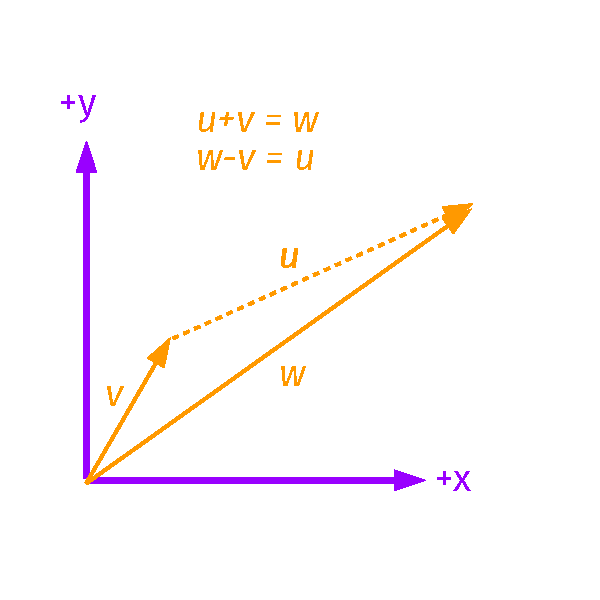
\includegraphics[width=0.45\textwidth]{figures/Vectors4.pdf}}
\subfloat[\label{fig:twovectors_b}]{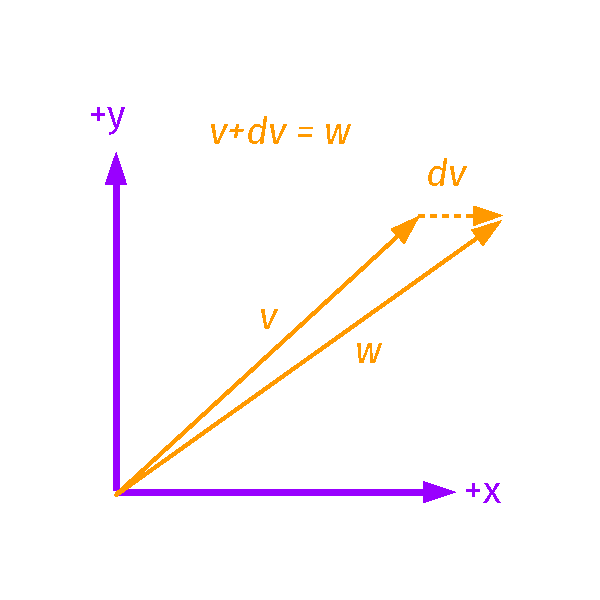
\includegraphics[width=0.45\textwidth]{figures/Vectors1.pdf}}
\caption{\label{fig:displacement} (Left): The displacement vector is $\vec{u}$.  (Right) Treat displacement for a small change in time, $dt$, and call it $dv$.}
\end{figure}
\end{frame}

\begin{frame}{Mathematics review: taking derivatives}
\small
\begin{minipage}[b]{0.45\linewidth}
Let $f(t) = A\sin(Bt) + Ct^2$.  \\ Compute $f'$. \\
\vspace{0.2cm}
\begin{itemize}
\item A: $f'(t) = AB\sin(Bt) + 2Ct$
\item B: $f'(t) = AB\cos(Bt) + 2C$
\item C: $f'(t) = AB\sin(Bt) + 2Ct$
\item D: $f'(t) = AB\cos(Bt) + 2Ct$
\end{itemize}
\end{minipage}
\hspace{0.5cm}
\begin{minipage}[b]{0.45\linewidth}
Let $f(t) = (4t-1)/(3t+2)$.  \\ Compute $f'$. \\
\begin{itemize}
\item A: $f'(t) = \frac{4}{3t+2}$
\item B: $f'(t) = \frac{4}{(3t+2)^2}+\frac{12t-3}{(3t+2)^2}$
\item C: $f'(t) = \frac{4}{3t+2}+\frac{12t-3}{(3t+2)^2}$
\item D: $f'(t) = \frac{12t-3}{(3t+2)^2}$
\end{itemize}
\end{minipage}
\end{frame}

\begin{frame}{Displacement, and instantaneous velocity and acceleration}
Definition of instantaneous velocity vector:
\begin{equation}
\boxed{v(t) = \frac{d\vec{v}}{dt}}
\end{equation} \\
\vspace{0.5cm}
Simple example: Let the vector position of an object be
\begin{equation}
\vec{x}(t) = (2t \hat{i} - 3t^2\hat{j}) \quad m
\end{equation}
Then
\begin{equation}
\vec{v}(t) = (2 \hat{i} - 6t\hat{j}) \quad m/s
\end{equation}
\end{frame}

\section{Answers}

\begin{frame}{Answers}
\begin{columns}[T]
\begin{column}{0.5\textwidth}
\begin{itemize}
\item $\vec{R} =  (-3\hat{i}-16\hat{j})$ m
\item 2 m$^2$
\item $f'(t) = AB\cos(Bt) + 2Ct$
\item $f'(t) = \frac{4}{3t+2}+\frac{12t-3}{(3t+2)^2}$
\end{itemize}
\end{column}
\begin{column}{0.5\textwidth}
\begin{itemize}
\item 
\end{itemize}
\end{column}
\end{columns}
\end{frame}

\end{document}
